%%%%%%%%%%%%%%%%%%%%%%%%%%%%%% -*- Mode: Latex -*- %%%%%%%%%%%%%%%%%%%%%%%%%%%%
%% project.tex -- 
%% Author          : Philip Johnson
%% Created On      : Tue Nov  4 10:26:48 1997
%% Last Modified By: 
%% Last Modified On: Thu Feb 01 15:37:16 2007
%% RCS: $Id$
%%%%%%%%%%%%%%%%%%%%%%%%%%%%%%%%%%%%%%%%%%%%%%%%%%%%%%%%%%%%%%%%%%%%%%%%%%%%%%%
%%   Copyright (C) 1997 Philip Johnson
%%%%%%%%%%%%%%%%%%%%%%%%%%%%%%%%%%%%%%%%%%%%%%%%%%%%%%%%%%%%%%%%%%%%%%%%%%%%%%%
%% 

\section{Introduction}

The goal of the Science of Design (SoD) program is to bring creative,
scientific advances to the design of software artifacts and systems.  New
paradigms, concepts, approaches, models, and theories arising from this
program should improve the processes of constructing, evaluating, and
modifying software-intensive systems. Important research questions include
the design and evaluation of software architectures with respect to their
quality and understandability; design optimization in the presence of
contradictory, inconsistent, emergent, and/or ambiguous requirements; and
analysis of tradeoffs between information and software design.  In all
cases the program focus is on basic research to advance the science of
software-intensive design, and on the effective application of SoD research
outcomes to the design of practical software intensive systems and their
integration into educational curricula.

The programmatic emphasis on ``creative'' approaches implies a preference
for revolutionary over evolutionary advances, and interdisciplinary over
single discipline approaches.  The programmatic emphasis on ``scientific''
approaches implies that the creativity should be framed within a
methodological context that supports, for example: (1) The ability to
characterize the internal and external validity of the findings; (2) The
ability to replicate the results; (3) Operational definitions for design
characteristics and outcomes relevant to the research, such as ``quality'',
``complexity'', ``performance'', ``usability'', ``maintainability'', and so
forth; and (4) Systematic measurement of qualitative and quantitative
metrics.

One impact of the Science of Design program results from the potential for
each project to discover one or more new design techniques with advantages
over the current state of the art in certain contexts of use.  This ``first
order'' impact could be augmented if at least some of these independent
findings are generated in a way that allows comparison,
combination, or meta-analysis with other findings.  This
facilitates  research on ``second-order'' impacts, such as
``Does the combination of new design technique X with new design technique
Y have an additive, multiplicative, or negative effect on software
quality?''  Comparability also accelerates the process of discovering the
context variables associated with research results, such as the types of
software or organizational contexts that support (or preclude) the use of a
new design technique.

A common way to facilitate direct comparison, combination, and
meta-analysis of data generated in separate research projects is through
the use of a testbed.  One approach to testbeds is a common artifact on
which multiple design techniques can be applied and the results compared.
For example, in the High Dependability Computing Project \cite{Boehm04},
the SCRover software was developed as a common artifact for assessing
different dependability techniques \cite{Boehm04b}. A second approach to
testbeds is an experimental infrastructure for standardized definition,
collection, and analysis of empirical measures. For example, the LDRA
Testbed uses both static and dynamic instrumentation for process
improvement, testing, and maintenance \cite{Hennel06}.  Both kinds of
testbeds are useful, and indeed complementary: you could use an
infrastructure testbed's instrumentation to gather process and product data
resulting from the application of design techniques to a common artifact
testbed.

To facilitate both first and second order impacts, the Science of
Design solicitation requests a special category of proposals focused on
``Demonstration Testbeds''.  These testbeds should support the development
of research infrastructures that enable evaluation of the utility and
quality of the artifacts produced by the Science of Design research
community.

In this project, we propose to perform research resulting in a new
infrastructure-oriented testbed called ``SoDeT'' (Science of Design
empirical Testbed), which will be based upon the Hackystat Framework
\cite{Hackystat}.  The open source Hackystat Framework has been under
development in our lab for five years and has been used in a wide variety
of research and industrial settings. Systems based upon the Hackystat
Framework involve the use of software ``sensors'' to capture both
``process'' and ``product'' data about the software under development.

By process data, we typically mean developer behaviors that can be detected
through their interaction with a tool.  For example, by instrumenting an
interactive development environment, Hackystat can detect developer
behaviors such as when code is compiled, unit tests are invoked, and so
forth.  Because Hackystat attaches timestamps to these events, it can
provide a record of the sequence of behaviors that occur.  SoDeT
will thus be able to measure design process data such as when an SoD
design tool is invoked, how long it is invoked for, and what other tools
were invoked (or not invoked) along with the design tool. 

By product data, we mean information produced by the invocation of analysis
tools on a software artifact.  This can include size or structural
complexity metrics; the count and types of quality assurance problems
detected by tools like Checkstyle, PMD, FindBugs; source evolution over
time as captured by the configuration management system; and so forth. 
SoDeT will thus be able to measure design product data generated by
SoD research, such as novel measures of design ``quality'', ``complexity'',
``efficiency'', or ``reliability''.

SoDeT will benefit from its ability to leverage existing Hackystat
support for over 30 sensors for a wide variety of programming languages and
tool frameworks.  For example, one SoD project focuses on a novel approach
to software testing and its interaction with design.  By instrumenting not
only to specific test tool developed by the SoD project, but also other
elements of the development environment, it becomes easier to investigate
``contextual'' questions, such as whether the SoD technique works within an
agile process such as Test Driven Design.

The SoDeT research project is designed with the goal of achieving the
following five objectives:

{\em 1. Provide a useful, usable demonstration testbed to a significant
number of Science of Design projects.} To achieve this objective, we have
already undertaken a preliminary feasibility study, the results of which are presented in
Section \ref{sec:preliminary-study}, and which we will build upon during the
project by a detailed feasibility study, as discussed in Section
\ref{sec:detailed-study}.

{\em 2. Improve the scientific benefits and research impact of individual
Science of Design projects.} The testbed will achieve this objective by
facilitating standard ways to define and collect outcome measures of interest to SoD
researchers, such as design ``quality'', ``reliability'', and ``cost''.
This improves the internal validity of the research, and facilitates replication
of SoD experiments in new contexts.  For example, Section \ref{sec:hackystat} describes an
example of a standardized measure called ``Active Time''.

{\em 3. Decrease the cost of empirical data collection and analysis for
design-oriented software research.}  By producing a useful, usable testbed
for Science of Design projects, a broader impact will be the creation of an
open source empirical infrastructure that should be helpful beyond the SoD
community to any design-oriented research efforts involving empirical
evaluation. Section \ref{sec:hackystat} discusses the trade-offs associated with 
automated vs. manual empirical data collection.

{\em 4. Facilitate comparative and meta-analysis of individual
projects.} As noted above, the impact of the Science of Design program will
be amplified if individual research projects generate results in a form
amenable to comparison, combination, or statistical meta-analysis with at
least some of the other projects.  By providing standardized data
definition and collection mechanisms, SoDeT can facilitate the integration
of individual results. Section \ref{sec:metaanalysis} describes our prior
experience with integrating together results from independent experiments
on software review.

{\em 5. Facilitate discovery of high impact ``second order'' research
opportunities.}  Also as noted above, an important future research
direction is to assess the opportunities that result from combining
individual research advances.  SoDeT is designed to both help in the
discovery of potentially useful combinations, as well as provide a
framework that can facilitate understanding and assessment of the outcome
of combining various techniques together.

The next section of this proposal presents a study of current SoD projects
that was undertaken in order to assess the feasibility of SoDeT.  The
following section presents related work, including the Hackystat Framework
and its relationship to other forms of testbeds.  We next present our plan
for how we intend to facilitate voluntary adoption of SoDeT by
SoD participants. We conclude with a summary of the intellectual merit and broader
impacts of this research project.

\section{A preliminary feasibility study}
\label{sec:preliminary-study}

\begin{figure*}[t]
\small
\begin{tabular}{|p{0.70in}|p{1.85in}|p{1.85in}|p{1.85in}|} \hline
{\bf PI(s)/ \newline (Response)} & {\bf Project Focus} & {\bf Tools Produced} & {\bf Outcome Measures/Hypotheses} \\ \hline

Abdelwahed (+)&
Model-based real-time, \newline  embedded system design &
Model-based design, analysis, \newline verification tools  &
(Improved) design, \newline (Improved) implementation \\ \hline

Amoussou &
Design Education &
None indicated &
None indicated  \\ \hline

Bailey &
Early stage UI design &
Visual sketching language, Early stage creative design tool &
None indicated  \\ \hline


Basili, \newline Carver (-)&
Architectural change management &
None indicated  &
Models of architectural change, faults, design \\ \hline

Batory &
Generative Programming &
None indicated &
(Improved) program synthesis, optimization, and evolution \\ \hline

Bodik (+)&
Programming by sketching &
Sketching Synthesizer for Scientific Programs &
None indicated \\ \hline

Boehm (+)&
Value-based design &
Value-based software design tools &
None indicated \\ \hline

Bultan &
Design for Verification &
None indicated &
None indicated \\ \hline

Devanbu &
Open source design &
None indicated &
None indicated  \\ \hline

Ernst (-)&
Software design and testing &
Test generation from designs &
(Improved) execution, \newline (Improved) coverage \\ \hline

Findler \newline Felleisen &
Software markets, quality assurance, and design &
None indicated &
None indicated \\ \hline

\end{tabular} 
\caption{Feasibility of SoD projects for SoDeT adoption (Part 1 of 4)}
\label{fig:sod-1}
\normalsize
\end{figure*}

\begin{figure*}[ht]
\small
\begin{tabular}{|p{0.70in}|p{1.85in}|p{1.85in}|p{1.85in}|} \hline
{\bf PI(s)/ \newline (Response)} & {\bf Project Focus} & {\bf Tools Produced} & {\bf Outcome Measures/Hypotheses} \\ \hline

Fischer &
Participative software design &
Meta-design framework &
(Improved) participation \\ \hline

Flanagan &
Ethics and politics in design &
Values-in-design toolkit &
None indicated \\ \hline

Flatt, \newline Shivers &
Language ``towers'' &
Meta-tools for language design &
(More efficient) language design \\ \hline

Gamboa &
Design comprehensibility &
Enhanced Daikon, \newline Enhanced AbsInt &
Design quality (comprehensibility) \\ \hline

Getoor &
Semantic data integration, transformation, and sharing &
Data viewers, mappers, transformation languages &
None indicated \\ \hline

Goel &
Teleological Reasoning in Design &
Interactive software design environment &
Efficacy of teleological-based design  \\ \hline

Guzdial &
End-user programming &
None indicated &
None indicated \\ \hline

Hicks (+)&
Software Design Evaluation &
Tools for software design evaluation &
None indicated \\ \hline

Jackson \newline Perry (+)&
``Prescriptive'' software architecture descriptions &
Alloy constraint system \newline Compositional Compiler  &
(Improved) design quality \newline (Improved) design trade-offs \\ \hline

Jagadish (-)&
Incremental design of XML information systems &
Automated mapping/translation of schema &
(Reduced) effort to design and maintain information stores \\ \hline

Klein &
Non-linear negotiation for design &
Taxonomic knowledge base of designs &
(Improved) component choice, \newline (Improved) design efficiency \\ \hline

\end{tabular} 
\caption{Feasibility of SoD projects for SoDeT adoption (Part 2 of 4)}
\label{fig:sod-2}
\normalsize
\end{figure*}

\begin{figure*}[ht]
\small
\begin{tabular}{|p{0.70in}|p{1.85in}|p{1.85in}|p{1.85in}|} \hline
{\bf PI(s)/ \newline (Response)} & {\bf Project Focus} & {\bf Tools Produced} & {\bf Outcome Measures/ \newline Hypotheses} \\ \hline

Liu \newline Stoller &
Reconciling modularity and efficiency &
Language for design knowledge &
Design invariants \\ \hline

Lorenz \newline Attie &
Design locality &
``Pairwise composition'' analysis and verification tools &
Modular, modifiable, and maintainable designs \\ \hline

Mok \newline Abdelzaher &
Embedded software design &
Feedback control and stability tools &
(Improved) reliability \newline (Reduced) cost \\ \hline

Paul &
Multiprocessor chip design &
None indicated. &
None indicated \\ \hline

Rajlich &
Design of incremental change &
Static program analysis &
(Improved) quality \newline (Reduced) maintenance costs \\ \hline


Reiss &
Semantic component design &
None indicated &
(More controllable) design \\ \hline

Robinson (+)&
Requirements Monitoring, \newline End-user goals &
Run-time compliance monitor &
None indicated \\ \hline

Roth (+)&
Learning based programming &
Hybrid imperative/machine-learning language &
(Better) programming abstractions \\ \hline


Shaw &
Managing uncertainty in design &
None indicated &
(Reduced) user uncertainty \\ \hline

Sheard &
Semantics-based system design &
Omega &
None indicated  \\ \hline

Shipman &
Design by end-user &
End-user design tool \newline Design Repository &
(Improved) stakeholder communication, involvement \\ \hline


\end{tabular} 
\caption{Feasibility of SoD Projects for SoDeT adoption (Part 3 of 4)}
\label{fig:sod-3}
\normalsize
\end{figure*}

\begin{figure*}[ht]
\small
\begin{tabular}{|p{0.75in}|p{1.85in}|p{1.85in}|p{1.85in}|} \hline
{\bf PI(s)/ \newline (Response)} & {\bf Project Focus} & {\bf Tools Produced} & {\bf Outcome Measures/ \newline Hypotheses} \\ \hline

Sreenivas &
Design of discrete event system supervisory policies &
None indicated &
(Improved) discrete event system designs \\ \hline

Siskind (-)&
Functional programming &
None indicated &
None indicated \\ \hline

Su &
Business Process Specification &
Business Process Design, \newline Business Process Management &
(Reduced) development time, \newline (Improved) code quality \\ \hline

Sullivan \newline Griswold  (+)&
Economic analysis of design &
None indicated &
Economic ``value'' of designs \\ \hline

Taha &
Synthesizing device drivers &
MetaOCaml &
(Improved) design process \\ \hline

Tanimoto (+)&
Collaborative Design &
Communication,  evaluation tools, T-Star &
None indicated \\ \hline

Taylor (-) &
Architectural Design &
Tools for applying ``proven'' architectural styles &
None indicated \\ \hline


Vardi &
Automated design &
Assertion based automated design tool &
(Higher) quality, \newline (Shorter) design cycles \\ \hline

Xie &
Feedback-based architectures &
Tools for mission-critical software &
(Improved) reliability, \newline (Reduced) cost \\ \hline

Zhou &
Design and specification with imperfect components &
Model-based analyzer, verifier &
Functional limits of feasible systems \\ \hline

\end{tabular} 
\caption{Feasibility of SoD projects for SoDeT Adoption (part 4 of 4)}
\label{fig:sod-4}
\normalsize
\end{figure*}

Given that there are at least two fundamentally different approaches to
testbeds (artifact-oriented and infrastructure-oriented), and a wide variety of different
projects being pursued in the Science of Design program, a basic question
for any testbed is: ``If you build it, will they come?''  In other words,
given that it is unlikely (and probably undesirable) for a single SoD
testbed to be mandated for use by all SoD projects, what is the likelihood
that a significant number of SoD projects will voluntarily adopt an SoD
testbed for use in their research?

Based upon our experience with external adoption of Hackystat over the past
several years, we believe that the answer to this question will depend upon two
properties of a testbed: utility and usability.  The utility of a testbed
concerns the degree to which it provides support for answering the research
questions of interest to the project leaders.  In the case of SoDeT, the
utility question for an SoD project leader translates to, ``Can SoDeT
gather process and product metrics that helps me answer interesting
questions about my design innovation?''

Even if a testbed has potential utility to an SoD project, it will not be
adopted unless it has an adequate level of usability.  Usability refers to
the level of effort required to install, configure, and use the testbed.
In the case of SoDeT, the usability question for an SoD project leader
translates to, ``How much time will be required from me or my staff to
install SoDeT, configure it for use in my project, gather the data,
and interpret the results?''

To provide some initial insight into the utility question with respect to
SoDeT, we searched the NSF Awards database for all currently
funded Science of Design awards. After eliminating awards for workshops and
consolidating multiple awards for team-based projects, we were left with 43
distinct projects. For these 43 projects, we reviewed the project abstract
to see if we could answer the following questions: (1) 
what kinds of design tools would be produced from the project, if any; (2)
what kinds of ``outcomes'' would be produced by the project, and (3)
whether the project abstract contained reference to any testable, empirical
hypotheses, such as ``improved'' quality or ``decreased'' cost?

Since the Awards database results included the PI name and contact email,
we also sent an email to each PI to gather more direct information about
the project.  In our email, we briefly introduced the SoDeT
approach and asked two questions: (1) would their research produce a
tool that appeared to be amenable to our form of testbed instrumentation,
and (2) would their research produce an empirical measure of one or more
design or implementation characteristics, such as ``quality'',
``goodness'', ``faults'', ``efficiency'', and so forth?

Figures \ref{fig:sod-1}, \ref{fig:sod-2}, \ref{fig:sod-3}, and
\ref{fig:sod-4} contain a summary of the results of our award abstract
review and email request to the PIs. (The projects are listed in
alphabetical order by PI name. The results are split into four tables
to improve page layout.)  The first column contains the name(s) of
the PI(s).  It also contains a ``(+)'' if a PI replied to our email with a
generally positive response concerning our two questions, and a ``(-)'' if
a PI replied with a generally negative response.  We received responses
to our email from 14 of the 43 projects (33\%).

The second column presents a phrase summarizing the focus of the project
based upon our review of the abstract.  The third column lists the tools
produced by the project, or ``None indicated'' if the abstract did not
indicate that tools would be produced.  The fourth column lists measurable
outcomes mentioned in the abstract if the research is successful.  If the
abstract indicates a testable hypothesis, the fourth column indicates that
using a parenthesized adjective, such as ``(Improved)'', ``(Reduced)'',
``(Higher)'', ``(Shorter)'', and so forth.

Before beginning the interpretation of this data, it is important to
understand the limitations of this preliminary feasibility study.
First, it is not possible to gain deep insight into a project from a one
paragraph description.  This means that we may have misconstrued the
presence/absence of tools or outcomes for certain projects.  In the same
way, since our email contained only a one paragraph description of the
SoDeT approach, it is possible that the responding PIs may have
been inappropriately positive (or negative) concerning its applicability to
their research.  Nevertheless, while we accept that there is considerable
uncertainty with respect to the correctness of our analysis of any
individual project, we hope that the aggregate analyses will provide at
least coarse evidence regarding the degree of compatibility between the
SoDeT approach and the Science of Design program as a whole. 

To begin, one capability of SoDeT is tool instrumentation,
which can simplify collection of data such as when a tool is invoked, the
outcome of the tool's invocation, the amount of time spent executing the
tool, and so forth.  If an SoD project does not produce a tool, then it is
less likely that this kind of data will be of interest.  From our analysis,
30 of the 43 project abstracts (70\%) indicate that a tool would be
produced as part of the research.  Thus, a substantial number of projects
at least qualify for tool instrumentation, though it remains unclear as to
whether SoDeT tool data would provide the project leaders with useful
insight regarding their research questions.

A second capability of SoDeT is to provide standard, operational
definitions for measures and a consistent framework with which to collect
and analyze them.  For example, five of the project abstracts include the
same testable hypothesis: that their tools and techniques will result in
``improved design quality''.  Of course, there are many different
definitions for ``quality'', many different types of artifacts that could
be considered a ``design'', and many different levels of ``improvement''.
The goal of SoDeT is {\em not} to coerce different projects
to agree to use the same measures.  Instead, the goal is for the framework
to be both sufficiently flexible and powerful so that project leaders can
define and collect the measures of interest to them more easily than they
could by ``handrolling'' their own measurement infrastructure.  If that is
accomplished, then use of the framework results a more precise
understanding of the differences between the measures designed by each
project, and creates opportunities for meaningful meta-analysis.  From our
analysis, 19 of the 43 project abstracts (44\%) included a potentially
testable hypothesis, and 26 out of 43 project abstracts (60\%) included
either a potentially testable hypothesis or an empirical outcome measure.

In summary, looking at the Tool column alone indicates 70\% of the projects
are potentially appropriate, and looking at the Outcome column alone
indicates that 60\% of the projects are potentially appropriate.  If this
analysis approach is appropriate, then we would predict that projects
designed to produce both a tool and an outcome measure or hypothesis would
be the most likely to be amenable to SoDeT.  We would likewise
predict that projects producing neither a tool nor an outcome measure or
hypothesis would be least likely to be interested.  The tables reveal that
20 out of 43 project abstracts (47\%) mention both a tool and an outcome,
16 out of 43 project abstracts (37\%) mention either a tool or an outcome,
and the remaining 7 project abstracts (16\%) mention neither a tool nor an
outcome.

The email responses from PIs are generally consistent with these
percentages: 9 out of 14 replies (64\%) indicated a potential interest in
applying the SoDeT approach to their project.  Unfortunately, the
project abstract analysis results and the email results are not entirely
consistent.  For example, two of the five negative email responses came
from projects whose abstracts indicate that they will produce both a tool
and an outcome.  The other three had at least one ``None indicated'' for
their tool or outcome.

The preceding feasibility analysis addresses only the ``utility'' question;
it does not provide insight into the ``usability'' of SoDeT.  Some
indirect insight into SoDeT usability can be inferred from usability
research on the Hackystat Framework \cite{csdl2-03-12,csdl2-07-02}.  The
first study revealed problems with client-side installation of sensors,
which was addressed through a client-side GUI installer wizard.  The latest
usability study of Hackystat has initiated a redesign of its server-side
web application user interface to incorporate Ajax and other ``Web 2.0''
features.  Despite these issues, Hackystat is currently usable enough for
application in a variety of academic and industrial contexts, as discussed
in Section \ref{sec:hackystat}.

In conclusion, this preliminary feasibility analysis appears to indicate
that, based upon project abstracts, the testbed approach embodied by SoDeT
is feasible from a utility point of view to slightly less than half of the
current SoD projects.  If we assume that, in a similar way, slightly less
than half of those projects find SoDeT to be adequately usable, then SoDeT
will be adopted by approximately 9 SoD projects.  If we use the email reply
percentage as a basis, then we get the more optimistic adoption estimate of
18 projects.

\section{Related Work}

\subsection{Artifact and infrastructure testbeds}

As discussed above, there are two common approaches to research
testbeds. One approach is artifact-centered, focusing on a software
implementation that is suitable for use in multiple research contexts.
Another approach is infrastructure-centered, focusing on a framework for
consistent monitoring and measurement independent of a specific software
artifact.  These approaches can be implemented independently or combined
\cite{Lindvall05}.

The High Dependability Computing Project produced two artifact-centered
testbeds: the Inspector SCRover \cite{Boehm04b} and the TSAFE air
traffic control support system \cite{Dennis03}.  In both cases, the
testbeds provided access to the source code of the systems along with
documentation, seeded defects, instrumentation techniques, and guidelines
for experimental use.

As an example of how an artifact-centered testbed is used, a version of the
SCRover software was seeded with 24 defects and then subjected to
dependability analysis using the MAE environment for functional
architecture specification based upon xADL \cite{Dashofy02}.  Applying MAE
to the SCRover testbed resulted in it finding 15 of the 24 seeded defects,
plus 6 additional defects not previously known in the software.  A similar
form of analysis was carried out using ACME ADL \cite{Garlan00}, a
different approach to architectural specification and analysis.  Comparing
the two approaches found that each approach found certain types of defects
not found by the other, that both found defects not known beforehand
(i.e. not present as a seeded defect), and that combining the two
approaches could be both feasible and advantageous \cite{Boehm04b}.

Leap \cite{csdl2-00-03}, Hackystat \cite{Hackystat}, LDRA \cite{Hennel06},
EPM \cite{EPM}, PROM \cite{PROM}, ECG \cite{ECG}, and SUMS \cite{SUMS} are
all examples of infrastructure-centered testbeds.  In these systems, no
single software artifact is specified.  The focus is instead on how to
consistently and effectively capture product and process characteristics of
whatever artifact is under development.  The infrastructures also focus on
lowering the cost associated with measurement collection and analysis.

Examination of infrastructure testbeds reveal various design trade-offs.
Some testbeds, such as SUMS, provide instrumentation at the operating
system level, and can reliably detect low-level events such as window focus
events and network traffic, but are not well-suited to detecting specific
behaviors with a development tool, such as the invocation of a refactoring
command from a menu.  Other testbeds, such as Hackystat and EPM, provide
instrumentation at the tool level.  The benefit of this approach is that
tool-specific behaviors can be captured, but the cost is that
instrumentation software must be individually developed for each tool of
interest.

As an example of how an infrastructure-centered testbed can be used, the
Leap toolkit was used to compare 13 different analytical methods for time
and size estimation \cite{csdl2-00-03}.  The results enabled direct
comparison of the accuracy of methods such as the PROBE method from the
Personal Software Process to a variety of regression models as well as
developer ``guesstimation''.

\subsection{Hackystat}
\label{sec:hackystat}

SoDeT will be implemented using the Hackystat Framework, which
provides an infrastructure for automated software development process and
product metric collection.  Hackystat includes a variety of features useful
for SoDeT, including unobtrusive, sensor-based data collection, 
platform and tool independence, open source licensing, integration with
visualization packages such as JFreeChart and statistical analysis packages
such as R, support for both individual and group-based software development, 
and experiment management services. 

Hackystat is a relatively mature open source project, with approximately 50
stable releases spanning five years of development, and over 300,000 lines
of source code. Data collection sensors are available for over 30 tools
including Eclipse, Emacs, JBuilder, Jupiter, Jira, Visual Studio, Ant,
JUnit, JBlanket, CCCC, DependencyFinder, Harvest, LOCC, Office, CVS, and
SVN.  

Hackystat is being used in a variety of academic and industrial contexts.
At the University of Hawaii, Hackystat is integrated into the undergraduate
and graduate software engineering curriculum, and is used by approximately
50 students per year to provide experience in empirically-based software
project management \cite{csdl2-03-12}. It has been used at NASA's Jet
Propulsion Lab to analyze the daily build process for the Mission Data
System \cite{csdl2-03-07}.  Hackystat is used as a testbed for collecting
and analyzing developer productivity data by researchers at the University
of Maryland and SUN Microsystems as part of the DARPA High Productivity
Computing Systems program \cite{Hochstein05,csdl2-04-03,csdl2-04-22}.
Finally, Hackystat is actively used in industrial settings, including
software development groups at Expedia, Teradata, Motorola, Applied Systems
Intelligence, InfoSys, Wolters Kluwer, and other companies.

To provide a concrete sense for how SoDeT can be applied to SoD projects,
the following sections overview four examples of testbed capabilities and
how the Hackystat Framework currently supports them: (1) measuring
developer effort; (2) process compliance, (3) longitudinal studies, and (4)
experiment management.   

{\em Effort measurement.} Consistent and reliable measurement of developer
``effort'' has long been a methodological problem for software engineering
research.  One approach is direct observation, in which the researcher
observes the developers and records their activities and elapsed time spent
on each.  The problems with this method are: it is too labor-intensive to
employ for extended periods; different researchers might not record data
consistently; and developers might change their work habits during the time
of the observation due to the presence of observation.

A second approach is to use developer logs.  Developers logs are
inexpensive to collect, but self-reported effort data can be inaccurate for
a variety of reasons, ranging from inaccurate recall to deliberate
misreporting for social or political reasons \cite{Hochstein05}.

A third approach is automated measurement of effort. For example, Hackystat provides the 
``DevEvent'' sensor data type to collect data on programmer
behaviors while performing tasks, and can be used in analyses that derive a
variety of measures for ``effort''.  For example, the ``Active Time''
measure represents the time spent while modifying the files related to the
project under development.  The measure is implemented using IDE sensors
with a timer-based process that wakes up periodically (30 seconds is the
default), checks whether the active buffer has changed since the last
check, and if so generates a ``State Change'' DevEvent.  The Active Time
measure partitions each day into 288 five minute chunks, and allocates five
minutes of Active Time to the developer if any ``State Change'' DevEvents
have occurred within the given time chunk.  Sensitivity analysis has
provided evidence that this five minute chunk size is appropriate for
accurately representing overall Active Time \cite{csdl2-02-09}. Most
importantly, Active Time can be measured consistently and reliably for many
different tools including Emacs, Eclipse, Visual Studio, JBuilder, and
IntelliJ Idea.  This allows direct comparison, aggregation, and
meta-analysis of Active Time measurements.

The principal disadvantage to automated measurement of effort is that it is
inherently incomplete: developers certainly exert ``effort'' during
meetings or phone calls that do not result in sensor data generation and
collection.  However, while certain kinds of efforts are not captured, the
DevEvent/DevTime approach shows how to capture a subset of data
consistently, reliably, and unobtrusively.

This example, while simple, illustrates important testbed measurement and
analysis capabilities in SoDeT.  The DevEvent sensor data type illustrates
how SoDeT can represent low-level measures in a consistent manner across a
variety of tools.  Furthermore, the Active Time analysis is based upon a
standard algorithm for both collection and analysis of the DevEvent measures.
SoDeT can leverage this approach in three ways. First, it allows a credible
approach to comparing data collected from different tools and investigating
questions such as whether the use of design technique A (requiring Tool A)
requires less Active Time than design technique B (requiring Tool B).  Second,
it allows data from different tools to be aggregated together. Thus, one
can sum the Active Time measures gathered from multiple tools to gain a
credible perspective on the overall Active Time required for a given
combination of design techniques. Finally, it can enable meta-analyses in
which Active Time data from different experiments are aggregated together.

{\em Process compliance.}  A second hard problem for empirical software
engineering research is to determine whether developers are actually doing
what they say they are doing (or are ``supposed'' to be doing).  For
example, research on the Test Driven Design (TDD) process has identified
process compliance as a significant impediment to experimental validity:
different researchers might define TDD differently, and some experimental
designs rely on developer's self-reported data as to whether they are using
TDD \cite{Janzen:05, Wang:04}.

As with effort measurement, the standard approaches to process compliance
involve direct observation, developer logs, or automated mechanisms, each with 
similar strengths and weaknesses. 

In the Zorro Project \cite{csdl2-06-02}, we designed and implemented a
system based on the Hackystat Framework to infer whether, and to what
extent, developers are using test driven design practices during
development. The system includes custom sensors for Eclipse and Visual
Studio that gathers a variety of low level ``micro-process'' data,
including compilation, refactoring, unit test, and other code editing
events.  This stream of development events is partitioned into
``episodes'', which are then input to a rule-based system that classifies
them into one of 22 episode types, and finally determines whether each
episode corresponds to the TDD practice.  The Zorro Project illustrates a
practical technique for assessing process compliance of a design technique
which allows for ``shades of gray''. TDD process compliance is measured as
the percentage of episodes that are TDD, and so one can determine that a
developer used TDD practices 83\% of the time.  The Zorro Project has also
revealed that the TDD process is much more sophisticated than the simple
three phase ``red-green-refactor'' process used in textbooks.  The 22
``phases'' (episode types) in Zorro have emerged from validation activities
with expert TDD practitioners. 

Figure \ref{fig:Analysis-Table} illustrates how the Zorro system extracts
certain events from Eclipse or Visual Studio, classifies them, and can even
provide an explanation of its inferencing process for validation purposes.

\begin{figure*}[th]
  \center
  \includegraphics[width=1.0\textwidth]{zorro-episode-interface.eps}
  \caption{Zorro Classification Analysis}
  \label{fig:Analysis-Table}
\end{figure*} 

SoDeT can leverage process compliance techniques from the Zorro project to 
help understand SoD design innovations in at least two ways.  First, for
new design techniques that require activities to be carried out in some kind
of ordered or partially order fashion, SoDeT can help assess whether subjects
complied with the method when attempting to carry out the new design technique. 
Second, even if the design technique does not appear to constrain the process
in any way, SoDeT can be used to assess, for example, if the inclusion of the
new design technique affects an existing design method in some way. For example, 
is the new design technique compatible with agile practices such as test driven 
design as operationalized by Zorro?


{\em Longitudinal studies.}  Some forms of SoD evaluation will employ short
duration experiments, such as classroom evaluation or experiments involving
up to a few hours of activity by a set of participants.  In addition to
supporting these cross-sectional studies, SoDeT will also support
longitudinal studies, in which participants are monitored over longer
periods of time.  This can be a powerful way to uncover interactions
between new design techniques and other process or product characteristics
over the course of development.

For example, Figure \ref{fig:telemetry-coverage} illustrates one such interaction
between a design technique (in this case, test-driven design) and a product
characteristic (in this case, test suite coverage).  Advocates of TDD have
claimed that a by-product of the TDD design practice is high coverage.  The
Hackystat telemetry chart shown in Figure \ref{fig:telemetry-coverage}
shows two descending trend lines over an actual seven week period of development,
illustrating that as the percentage of TDD-compliant episodes dropped, the
test case coverage of that system also dropped.  Longitudinal studies, such
as this one, typically do not provide the controls necessary to establish
causality, but nevetheless provide a valuable form of information about
real world practices that complement other forms of scientific inquiry.

\begin{figure*}[th]
  \center
  \includegraphics[width=0.65\textwidth]{telemetry-tdd-coverage.eps}
  \caption{Longitudinal study example: TDD and Coverage}
  \label{fig:telemetry-coverage}
\end{figure*} 


{\em Experiment management.}  For an infrastructure testbed to be useful, 
it must minimize its impact on the experimental setting itself.  In the case
of SoD research, both the usability and utility of the testbed are diminished
if the subjects must be provided with training in the use of the testbed 
infrastructure.  Ideally, the testbed is entirely in the background and no 
interaction with it is required by the subjects. 

SoDeT will leverage the experiment management package developed for the Hackystat
Framework which is designed to address exactly these issues.  The Experiment 
Manager provides support for three types of activities: configuration, monitoring,
and analysis.  Configuration support includes administrator facilities for defining
the set of subjects in an experiment, configuring their accounts, and installing
sensors.  Monitoring support includes client-side analyses to verify that data
is being collected from subjects, and server-side analyses to ensure that the server
is receiving and processing the data correctly.  Analysis support includes both 
built-in analyses to gain a preliminary sense for the data, as well as export
mechanisms to allow the researcher to import the data into other data analysis systems
such as R. 

\subsection{Comparative analysis, meta analysis, and evidence-based research}
\label{sec:metaanalysis}

It is a maxim of empirical research that no single study gives unequivocal
results.  To gain confidence that empirical results are real and not just
due to random variation, one must perform multiple studies and integrate
their results together to gain a broader, more general perspective on the
phenomena of interest. However, integrating multiple studies in a credible
way isn't simple.
 
A classic approach to understanding what several studies say about some
phenomenon is to conduct a literature review, qualitatively summarize
existing results, and manually synthesize them. The drawback of this
approach is that it lacks precise methods for combining different results.

The ``evidence-based'' paradigm from medical research provides a more
formal approach to this literature review process.  Kitchenham has been
leading the movement for evidence-based software engineering, organizing
workshops on this topic and publishing papers explaining the issues
involved in applying evidence-based research techniques to software
engineering \cite{Kitchenham04,Kitchenham04a}.  She and her collaborators
propose a five step method for evidence-based software engineering: (1)
Convert the need for information [about a software engineering practice]
into an answerable question; (2) Track down the best evidence available for
answering the question; (3) Critically appraise that evidence using
systematic review for its validity (closeness to the truth), impact (size
of the effect), and applicability (usefulness in software development
practice); (4) Integrate the critical appraisal with current software
engineering knowledge and stakeholder values [to support decision-making];
(5) Evaluate the effectiveness and efficiency in applying Steps 1-4 and
seek ways to improve them for next time.  While promising, application of
systematic reviews and the integration of empirical software engineering
data from multiple sources has been found to be challenging
\cite{Jedlitschka04}.

A statistical approach for integrating multiple studies is called
meta-analysis. This approach has two steps. First, the experimenters
attempt to reconcile the primary experiments -- i.e. define a common
framework with which to compare different studies.  This involves defining
common terms, hypotheses, and metrics, and characterizing key differences.
Next, the data from the primary experiments are transformed or recalculated
according to agreed upon definitions. In the second step the transformed
primary data is combined and reanalyzed.  Unfortunately, it is not always
clear when meta-analysis is appropriate, what statistical models should be
used, or when it is acceptable to combine data from disparate sources.

In joint research with Adam Porter \cite{csdl-97-02}, we performed a
comparative analysis of our own prior empirical studies of software review.
The studies had a similar motivation: to assess the true contributions of
meetings to software review. They differed in their designs, instruments,
review documents, procedures, and measurements. These differences prevented
the use of meta-analysis. Instead, we developed a common analysis framework
that resulted in five hypotheses that could be tested against both
experimental data sets individually.  In each case, both studies confirmed
or rejected the hypothesis in the same direction, increasing our confidence
in the generality of the findings.  Furthermore, the comparative analysis
of the methods employed provided insights into the design of useful
experimental research on software review, and suggested important next
steps for research.

Systematic reviews, the comparative analysis approach we performed with
Porter, and meta-analysis form a spectrum of approaches to integrating
multiple experimental outcomes to improve one's confidence in the
generality (also known as external validity) of the findings.  Systematic
reviews can be performed on literature alone, without direct access to the
original research or researchers. Our comparative analysis of software
review required the participation of the researchers and access to the
original data sets. SoDeT will facilitate not only the production of papers
amenable to systematic review, but also provide a common infrastructure for
experimental design and data collection that will allow not only
comparative analysis, but even true meta analysis, where data sets can be
merged prior to re-analysis.

\subsection{Results from prior NSF research}

\begin{tabular}{lp{4.5in}}

Award number: & CCF02-34568 \\
Program: & Highly Dependable Computing and Communication Systems Research\\
Amount: & \$638,000 \\
Period of support: & September 2002 to September 2007 \\
Title of Project: & Supporting development of highly dependable software through
continuous, automated, in-process, and individualized software measurement validation \\
Principal Investigator: & Philip M. Johnson \\
Selected Publications: & \cite{csdl2-04-22,csdl2-04-13,csdl2-04-11,csdl2-03-12,
csdl2-02-07,csdl2-03-07,csdl2-04-02,csdl2-04-04,csdl2-04-11,csdl2-06-07,csdl2-06-08,csdl2-06-13,csdl2-06-06}
\end{tabular} \\ %[3mm]

The general objective of this  research project is to design,
implement, and validate software measures within a development
infrastructure that supports the development of highly dependable software
systems.  Contributions of this research project include: (a) development
of a specialized configuration of Hackystat to automatically acquire build
and workflow data from the configuration management system for the Mission
Data System (MDS) project at Jet Propulsion Laboratory; (b) development of
analyses over MDS build and workflow data to support identification of
potential bottlenecks and process validation; (c) identification of
previous unknown variation within the MDS development process; (d)
development of a generalized approach to in-process, continuous measurement
validation called Software Project Telemetry, (e) substantial enhancements
to the open source Hackystat framework, improving its generality and
usability; (f) development of undergraduate and graduate software
engineering curriculum involving the use of Hackystat for automated
software engineering metrics collection and analysis; (g) support for 3
Ph.D., 6 M.S., and 3 B.S. degree students.


\section{Project Plan}

The SoDeT Project is organized into six phases: 
(1) Detailed feasibility analysis, (2) Testbed kickoff, (3) Testbed
implementation and enhancement, (4) Trial adoption, (5) Testbed
deployment, and (6) Testbed findings.  The following sections describe
the goals and activities of each phase.  

\subsection{Detailed feasibility analysis}
\label{sec:detailed-study}

One useful outcome of the preliminary feasibility analysis presented 
earlier in this proposal is that determining the utility and usability
of a given testbed for a given SoD project is difficult without detailed
knowledge of both the testbed and the project.  Our conclusions from the
project abstracts were based upon detailed knowledge of the testbed but
superficial knowledge of the project; conversely, the conclusions in the
email responses were based upon detailed knowledge of the project but
superficial knowledge of the testbed. 

The first stage of this project is therefore to perform a more detailed
feasibility analysis based upon detailed knowledge of both project and
testbed.  To do this, we will contact the current SoD award PIs, introduce
the SoDeT Project, and explain that we are conducting a feasibility
analysis of the testbed. We will then request that they provide us with a
copy of the 15 page ``Project Description'' section of their Science of
Design proposal as well as any other related research artifacts they
believe would be helpful in our effort.

Based upon this project description and any other related
artifacts, we will perform an analysis with three outcomes.

The first outcome will be a detailed, individual feasibility analysis of
SoDeT for each SoD project.  This feasibility analysis will be
provided back to the PI(s) of the corresponding project for review and
feedback.  This analysis will consider at least the following issues: (1)
what specific forms of process or product data could be collected by the
testbed that would appear to be useful to the project; (2) what specific
kinds of analyses could be performed upon this data that would appear to
provide relevant findings for the research project; (3) what kinds of
methodological impact the use of the testbed would have on the project,
such as changes to the experimental evaluation method; (4) a recommendation
from our perspective as to whether SoDeT appears to be worth
pursuing by the project; and (5) if worth pursuing, what would be the
appropriate initial step by the project leaders to evaluate for themselves
the utility and usefulness of SoDeT.  Through iteration with the PIs, we
will refine this analysis until it represents a consensus viewpoint on the 
feasibility of the testbed for each project. 

The second outcome will be a set of new requirements for SoDeT
which will be needed in order to maximize its utility and usability to the
SoD community.  We expect these requirements to include: (1) new types of
sensors for the tools developed by the community or used as part of their
research process; (2) new kinds of sensor data types to represent the novel
forms of design issues and representations produced by the project,
including qualitative data representations; (3) new forms of analyses which
might or might not build upon existing Hackystat applications such as
Software Project Telemetry or SDSA; and (4) new forms of interface to
support appropriate communication of the analyses to the researchers and/or
designers.

The third outcome will be a document proposing a set of new projects with
``second order'' Science of Design research impact.  The new projects will
focus on possible ways in which SoDeT could facilitate new
kinds of research that integrates together existing independent SoD
projects.  An example of a loosely coupled form of integration would be to
collect the same type of sensor data in the same way by the different
sensors attached to the design tools produced by different projects.
Subsequent processing by a common analysis would reveal similarities and
differences between the application of the two design tools, at least with
respect to this form of data.  It may also reveal interesting insights into
the differences between the two contexts of application of the two tools.

An example of a more tightly coupled form of integration would be a project
in which two or more instrumented design tools or techniques are available
for application within the same development context.  A variety of
interesting research questions can be posed within this environment. For
example, if the use of all the tools is mandated, what is the impact on
outcome measures such as quality or efficiency?  How is usage of the
various design tools interleaved?  What is the impact of these tools on the
usage of other tools?  If the use of all the tools is not mandated, which
tools are voluntarily employed, when are they used, and what are the
outcomes of their usage?  

\subsection{Testbed kickoff}

Once the detailed feasibility analysis is completed, SoDeT will
be formally introduced to the community at a ``Kickoff'' presentation.  If
the timing for the Kickoff coincides with the yearly SoD PI meeting, we
will request time to do it there, otherwise we will conduct an online
web-based presentation (``webinar'') using commercial tools available for
that purpose such as WebEx or GoToWebinar.  At that meeting, we will
present the results of the detailed feasibility analysis stage to the
entire community for review and feedback.  For those projects that have
agreed to take the next step in evaluating SoDeT for use, we will provide
information on what steps should be taken next. 

While we will present and solicit feedback on the ``second order'' research
impact projects, we do not expect any formal commitment to these projects
at such an early date in the testbed research process. Instead, the goal at
this point is to catalyze a dialogue within the community on what kinds of
second order impacts are desirable and feasible, and how to move toward
that kind of research over time.

\subsection{Testbed implementation and enhancement}

As soon as SoDeT requirements become available, we will begin implementing 
the enhancements required to the Hackystat framework to support the SoD
projects for which a consensus on feasibility was reached.  As SoDeT 
will leverage the Hackystat Framework, it is possible in best case
scenarios that only simple sensor and analysis enhancements will be required,
and for those projects a SoDeT configuration could be available within 
a few weeks.  

We expect that we will receive a steady stream of enhancement requests from the
SoD community over the course of the project, and that the implementation and
enhancement activities will be substantial and ongoing throughout the course of 
the project. 

\subsection{Trial adoption}

As a first step toward SoDeT usage, an SoD project will download and
install a configuration of SoDeT loaded with the sensors,
analyses, and user interface features appropriate to their research as
revealed during the detailed feasibility analysis.

This configuration will then be applied to a pilot study by the SoD project
members.  The goals of the pilot study are to enable the SoD project members to 
become familiar with the use of the testbed to collect and analysis data, and 
to help discover any additional requirements for use not found during the 
detailed feasibility analysis stage.  

\subsection{Testbed deployment}

If the trial adoption stage is completed successfully, the SoD project can
move into full deployment of the testbed to collect the process and product
data in a scientifically useful manner. For example, while the pilot study
phase might use members of the SoD project team itself for data collection,
this phase might use the testbed to collect data from students randomly
assigned to treatment groups, or from industrial users.

We anticipate that even during testbed deployment, the SoD projects will
uncover additional requirements and desirable enhancements to SoDeT, which
we will do our best to implement and distribute in a timely manner.

\subsection{Testbed findings}

In the final six months of the project, we will transition out of
development and support mode and into a findings phase with two primary
activities.

The first activity is the development of an ``Experience Base''
\cite{Basili94} that provides insights into the lessons we learned about the
development of a Science of Design testbed and its deployment in the
research program.  The goal is to provide transferable knowledge to other
NSF programs in which testbed infrastructure is desired, so that our
experience can be replicated with greater efficiency and impact.  The open
source SoDeT software will also be available as a reference to support this
tech transfer activity.

The second activity during this findings phase of the project is to
collaborate with the SoD PIs to refine and improve the initially proposed
set of ``second order'' research projects in light of the data and outcomes
of the individual projects.  The goal of this activity is to generate an
agenda for subsequent research in which comparison, replication, and
meta-analysis are explicit goals.

\subsection{Work breakdown structure}

Figure \ref{fig:wbs} provides a work breakdown structure that shows when
each of these phases begins and ends during the project and how they
overlap in time.  We split each year into two six month periods: ``Fall'' 
lasts from July to December, and ``Spring'' lasts from January until June.

\begin{figure*}[ht]
  \centering
  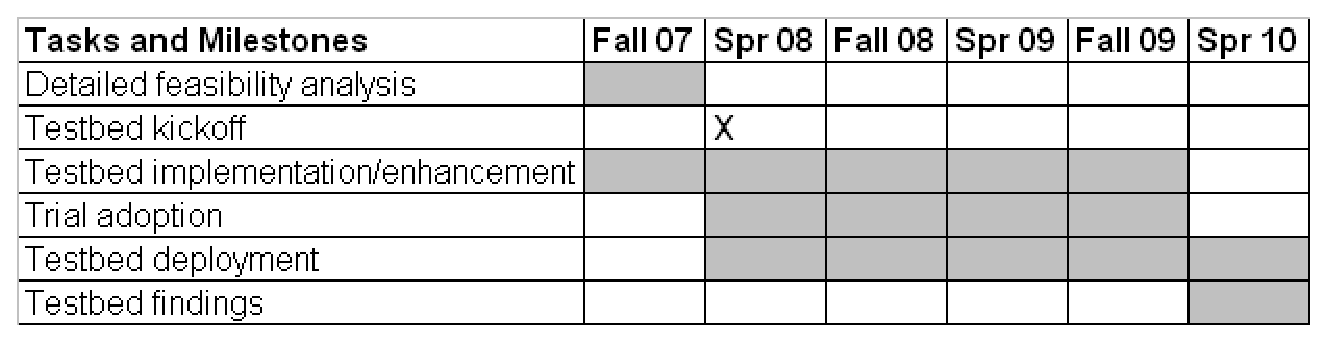
\includegraphics[width=0.75\textwidth]{workstructure.eps}
  \caption{Work breakdown structure and milestones.} 
  \label{fig:wbs}
\end{figure*}

Assuming that this project begins in Fall, 2007, we anticipate finishing the Detailed feasibility
analysis phase within six months.  This enables the Testbed kickoff meeting to occur in early 
Spring, 2008.  

Testbed implementation and enhancement will begin as soon as information begins to be available
as a result of the Detailed feasibility analysis, and will continue throughout the project until 
the last six months, at which point the focus will shift to ``wrapup'' activities. 

Trial adoption by participating SoD research groups should start in Spring 2008 and is expected
to continue for the next year or two.  We anticipate that for any individual research project,
the trial adoption phase will last a few weeks to a few months, but that research projects will
become ready to undergo Trial adoption at varying times over the course of this project.

Similarly, the Testbed deployment phase could start as soon as Spring 2008 for some SoD
projects, but could start as late as Spring 2010 for others.  The duration of the deployment 
phase for any given SoD research project is purely a function of their project and its goals. 
In some cases, the Testbed might be used for only a few weeks to conduct a controlled experiment, 
while others might use it for a longitudinal case study lasting many months. 

Finally, the Testbed findings phase will occupy the final six months of the project. 

\section{Conclusions}
\label{sec:merit}

NSF Science of Design proposals are evaluated according to their
intellectual merit, broader impacts, and new, creative ways to think about
a Science of Design discipline.

SoDeT has the potential to significantly advance knowledge and
understanding within the Science of Design program.  It can accomplish this
in several ways. For example, it will provide new, standardized, comparable ways
to operationalize the empirical measurement of design characteristics
produced by individual SoD projects.  This will both raise the quality of
research results from individual projects, and enable forms of
meta-analysis across multiple projects that might not have been possible
without a common framework for process and product data collection and
analysis.

Second, SoDeT will significantly reduce the cost to individual
researchers of data collection and analysis. Use of the testbed will reduce the
need by individual projects to develop custom data collection software, or
to alternatively employ manual data collection techniques, which are more
time-consuming, less scalable, and more error-prone.

Third, this year's solicitation expresses the desire to ``look forward in
the near future to the effective application of SoD research outcomes to
the design of practical software-intensive systems''.  SoDeT will be
designed to provide instrumentation support for laboratory, classroom, and
industrial environments.  It can thus facilitate more rapid technology
transfer of the design innovations from laboratory to ``real-world''
environments, providing high quality data back to the researchers that can
help them to recognize and respond to issues as they arise in new settings.

Fourth, our preliminary feasibility analysis provides evidence that a significant number of SoD
projects will find SoDet to be both useful and usable.

Finally, the SoDeT project will leverage the existing
Hackystat Framework along with the enhancements suggested by the detailed
feasibility analysis to produce a novel, creative approach to a
demonstration testbed that is uniquely suited to the Science of Design
discipline.

The broader impacts of this research project result from the fact that
SoDeT, being open source and based on the Hackystat Framework, will be
amenable to use in contexts outside of the Science of Design program. As an
open source project, SoDeT will be freely available for use and adaptation.

SoDeT can also improve educational opportunities in software
design.  The Hackystat Framework is used regularly in educational settings
to teach about software engineering measurement, and SoDeT
enhancements can be adapted to this environment to support teaching about
new design innovations and their impact upon design characteristics.

As the University of Hawaii is a university with 75\% minority students in
an EPSCOR state, a final broader impact of this project is the potential
for it to provide novel research opportunities to underrepresented groups.




